\documentclass[a4paper]{article}
\usepackage[slovene]{babel}
\usepackage[T1]{fontenc}
\usepackage[utf8]{inputenc}
\usepackage{lmodern}
\usepackage{amsfonts}
\usepackage{amsmath}
\usepackage{makeidx}
\usepackage{graphicx}
\graphicspath{ {./images/} }



\title{Finančni praktikum \\\vspace{2cm} {\huge $k$-total rainbow domination numer vs. domination number}\vspace{2cm}}
\author{Tim Resnik \\[1.5mm] Lana Herman \\[1.5mm]\vspace{6cm}
Univerza v Ljubljani \\[1.5mm]
Fakulteta za matematiko in fiziko \vspace{2cm}}
\date{November, 2019}

\begin{document}

\begin{titlepage}
\clearpage \maketitle
\thispagestyle{empty}
\end{titlepage}

\tableofcontents
\pagebreak

\section{Problem naloge}

V projektni nalogi se bova ukvarjala z domeno, ki se ukvarja s povezavo med 'k-rainbow total domination number' (označimo z $\gamma_{krt}(G)$)  in 'domination number' (označimo z $\gamma(G)$). Definiciji za $\gamma_{krt}(G)$ in $\gamma(G)$ sta v razdelku \textbf{Razlaga pojmov}.\\
Domneva pravi, da za graf G in $k \geq 4$ \text{obstaja tesna povezava} $\gamma_{krt}(G) \geq 2\gamma(G)$. Cilj najine projetkne naloge je najti tak graf, za katerega ta neenkost ne drži. To sva na majhnih grafih preverila na konkretnih primerih, kjer sva število vozlišč in število $k$ vnesla ročno. Za večje grafe sva uporabila metodo \textit{Simulated Annealing}.\\
Poiskala sva tudi primere, za katere velja enakost $\gamma_{krt}(G) = 2\gamma(G)$.

\section{Razlaga pojmov}

Graf $G$ ima množico vozlišč $V(G)$ in množico povezav $E(G)$. Za množico $N_G(v)$ velja, da vsebuje vsa sosednja vozlišča $v$, v grafu G. Za grafa G in H, je kartezični produkt $G \square H$ graf z množico vozlišč $V(G) \times V(H)$.\\
\textit{Dominirana množica} grafa $G$ je $D \subseteq V(G)$, taka da za vsako vozlišče $v \in V(G)$ in $v \notin D$ velja, da je sosed nekemu vozlišču iz $D$. \textit{Dominirano število}, $\gamma(G)$, je velikost najmanjše dominirane množice. Če za $\forall v \in V(G)$ velja, da je sosed vozlišču iz $D$, za $D$ rečemo, da je \textit{totalno dominirana množica} grafa $G$. \textit{Totalno dominirano število}, $\gamma_{t}(G)$, je velikost najmanjše totalno dominirane množice.\\
Za pozitivno celo število $k$, je \textit{'k-rainbow domination function'} ($k$RDF) grafa $G$ funkcija $f$, ki slika iz $V(G)$ v množico $\{1, \cdots, k\}$. Zanjo velja, da za katerikoli $v \in V(G)$ in $f(v) = \emptyset$ velja $\cup_{u \in N_G(v)} f(u) = [k]$. Definiramo $\|f\| = \sum_{v \in V(G)}|f(v)|$. $\|f\|$ rečemo \textit{teža} $f$-a. \textit{'k-rainbow domination number'}, $\gamma_{kr}(G)$, grafa $G$ je minimalna vrednost $\|f\|$ za vse 'k-rainbow domination functions'. Po definiciji vemo, da za vse $k \geq 1$ velja $$\gamma_{kr}(G) = \gamma(G \square K_k).$$
Graf $K_k$ predstavlja polni graf na $k$ vozliščih. Nazadnje definirajmo še \textit{'k-rainbow total domination function'} ($k$RTDF), katera se od 'k-rainbow domination function' razlikuje v dodatnem pogoju, ki zagotavlja, da če za $\forall v \in V(G)$ velja $f(v) = \{i\}$, potem obstaja tak $u \in N_G(v)$, da je $i \in f(u)$. \textit{'k-rainbow total domination number'}, $\gamma_{krt}(G)$, grafa $G$ je minimalna vrednost $\|f\|$ za vse 'k-rainbow total domination functions'. Tudi tu za vse $k \geq 1$ velja $$\gamma_{krt}(G) = \gamma_t(G \square K_k).$$
\pagebreak

\section{Reševanje problema}

\subsection{Majhni grafi}

Za majhne grafe sva definirala naslednjo pseudokodo.
\begin{figure}[h!]
    \centering
    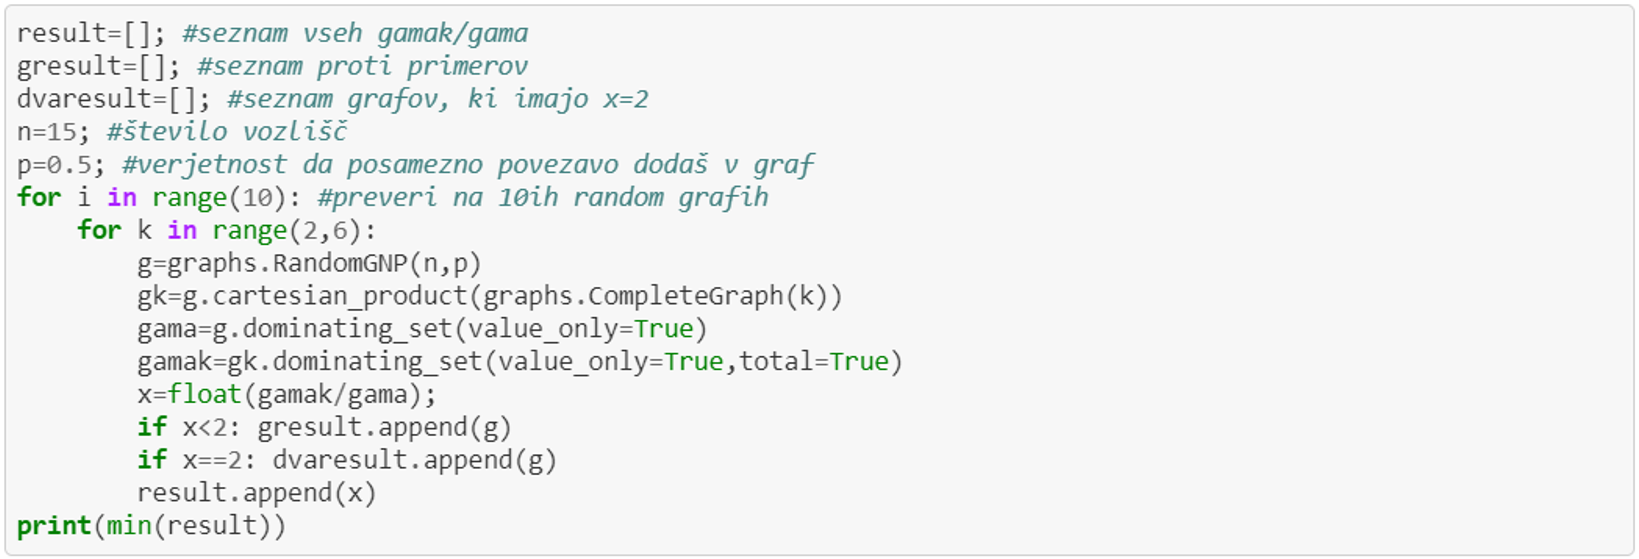
\includegraphics[width=13cm, height=5.35cm]{Slika1}
    \label{fig:mesh1}
\end{figure}\\
V kodi seznam \textit{result} predstavlja seznam vseh koeficientov $\frac{\gamma_{krt}(G)}{\gamma(G)}$, seznam \textit{gresult} predstvalja vse tiste grafe, za katere velja neenakost $\frac{\gamma_{krt}(G)}{\gamma(G)} < 2$, seznam \textit{dvaresult} pa predstavlja grafe za katere velja enakost $\frac{\gamma_{krt}(G)}{\gamma(G)} = 2$.\\
Prva zanka preteče $i$ naključnih grafov, generiranih z že vgrajeno funkcijo iz programa \textit{sage}, imenovano \textit{graphs.RandomGNP(n,p)}, kjer $n$ predstvalja število vozlišč, $p$ pa verjetnost, da posamezno povezavo doda v graf. Ta zanka je porabi $\mathcal{O}(n)$ časa.\\
Druga zanka se zapelje čez določeni število $k$-jev, kjer $k$ predstvalja število vozlišč na polnem grafu. Po definiciji namreč  vemo, da 'k-rainbow total domination number' izračunamo preko kartezičnega produkta med grafom $G$ in polnim grafom s $k$ vozlišči. Druga zanka porabi $\mathcal{O}(m)$ časa, kjer je $m$ število grafov, ki jih preteče $k$.\\
Funkcija \textit{cartesian\_product()} porabi $\mathcal{O}(n m)$ časa, saj vsakemu vozlišču iz grafa $G$ ($n$ vozlišč) priredi vsako vozlišče iz $k$-polnega grafa ($m$ vozlišč).\\
Torej je časovna zahtevnost te pseudokode enaka $\mathcal{O}(n^2 m^2)$.\\[1.5mm]
To kodo sva uporabila za $n \in \{5, \cdots, 20\}$ na različnem številu korakov in različnih $k$-jih. Za $k \geq 3$ sva minimum zmeraj dobila enak 2, za $k = 2$ pa sva dobila veliko protiprimerov, npr.:
\pagebreak
\begin{figure}[h!]
    \centering
    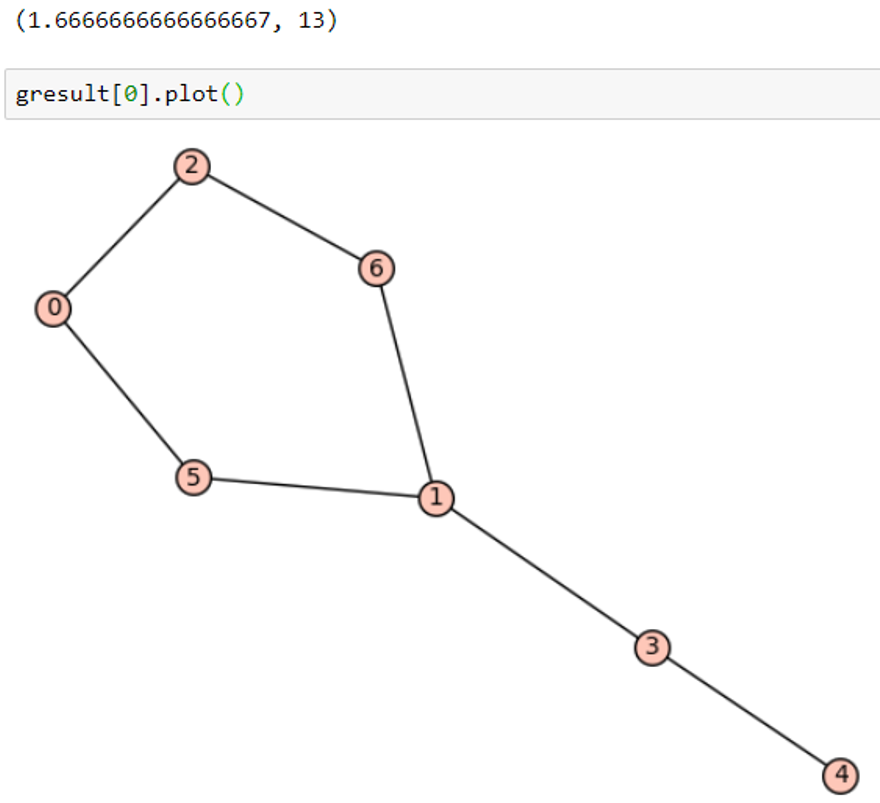
\includegraphics[width=7.5cm, height=6cm]{Slika2}
    \label{fig:mesh1}
\end{figure}\\
Opazimo, da je takih grafov kar 205 (koda je preverila na 1000 grafih s 15 vozlišči). To število se seveda spreminja, ko kodo poženemo večkrat. Zato sva jo pognala večrat in na različnem številu vozlišč. Vse skupaj je koda pregledala približno $10^{100}$ grafov, izključno za $k = 2$. Podatke sva izpisala v program \textit{Matlab}, jih za posamezno število vozlišč povprečila in jih aproksimirala z že vgrajeno funkcijo \textit{interp1}. Dobila sva spodnji graf.
\begin{figure}[h!]
    \centering
    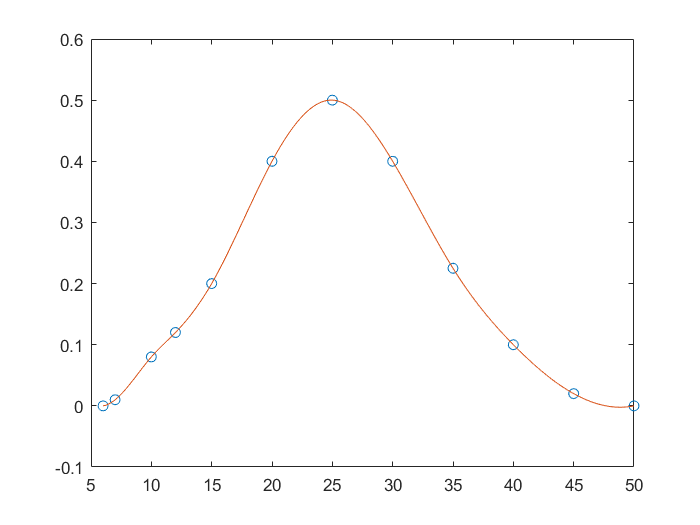
\includegraphics[width=7.5cm, height=6cm]{Slika3}
    \label{fig:mesh1}
\end{figure}\\
Opazimo, da protiprimerov ne dobimo za grafe z manj kot 7 vozlišč, za večje grafe pa velja, da gre število protiprimerov proti nič, ko se veča število vozlišč. Največ pa jih je pri grafih s približno 25 vozlišči.
\pagebreak

\subsection{Veliki grafi}

Za velike grafe sva definirala naslednjo pseudokodo.
\begin{figure}[h!]
    \centering
    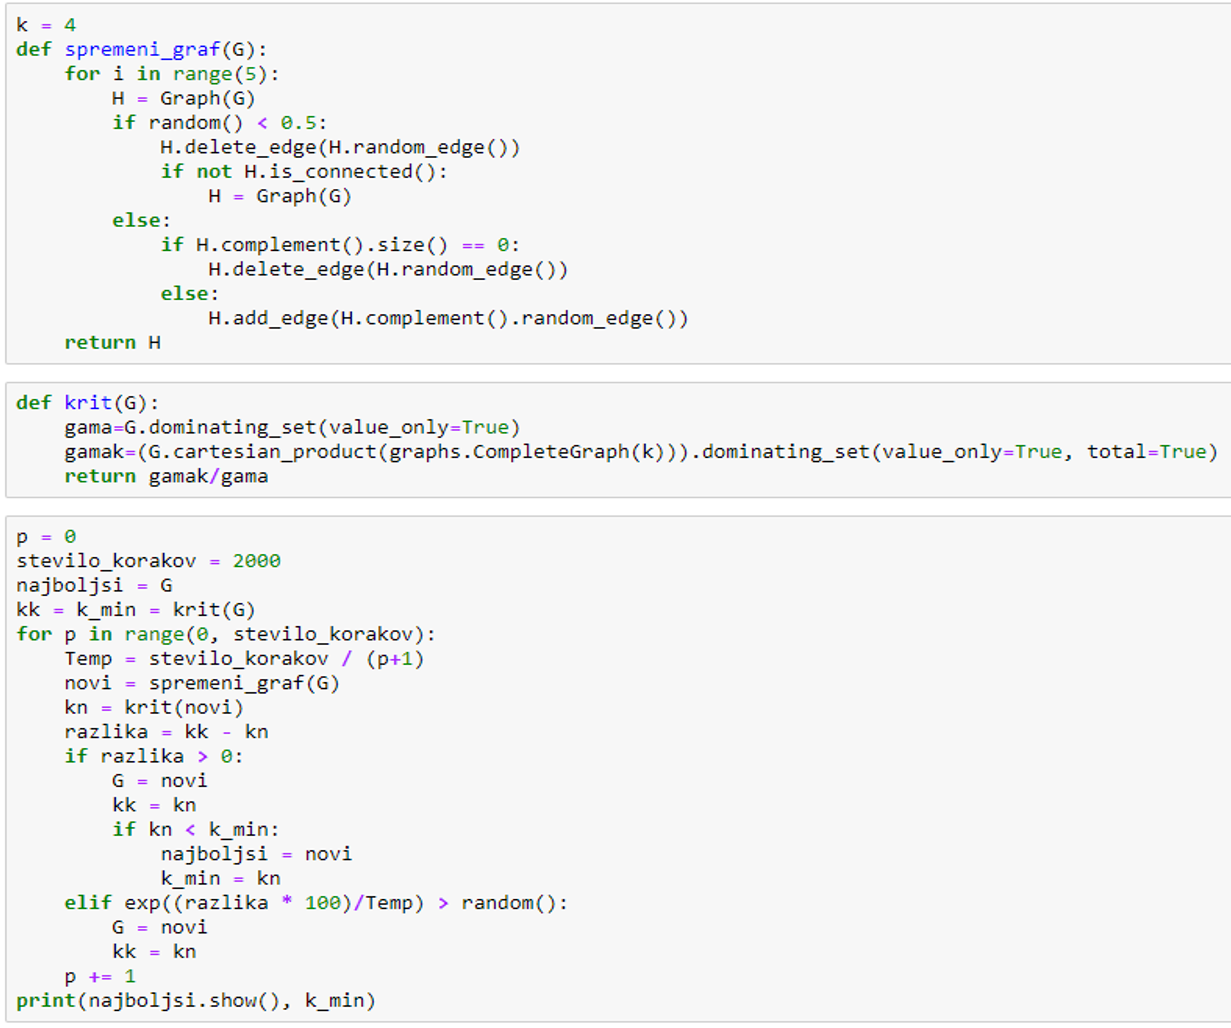
\includegraphics[width=13cm, height=11cm]{Slika4}
    \label{fig:mesh1}
\end{figure}\\
Funkcija \textit{spremeni\_graf()} nam ne nepovezan graf tako spremeni, da mu naključno odstrani povezavo in naključno doda povezavo. To funkcijo sva definirala zato, da sva jo lahko uporabila v naslenji kodi. Njena časovna zahtevnost je $\mathcal{O}(n^2)$, saj gre čez dve for zanki, vsaka ima zahtevnost $\mathcal{O}(n)$.\\
Zadnja koda pa predstavlja metodo \textit{Simulated Annealing}. To je metoda za približevanje h globalnemu optimumu dane funkcije. Tako sva s spreminjanjem danega grafa iskala tak graf, za katerega bo veljalo $\frac{\gamma_{krt}(G)}{\gamma(G)} < 2$. To kodo sva pognala na grafih z vsaj 20 vozlišči. Na podlagi najinih poizkusov sva ugotovila, da za grafe s sodim številom vozlišč, za vsak $k \ge 4$, je koeficient enak 2 , za grafe z lihim številom vozlišč pa sva domnevala, po nekaterih poizkusih iz manjših grafov, da velja formula $\frac{n}{\lfloor{\frac{n}{2}}\rfloor}$. Potem sva pognala kodo na grafu z neparnim številom vozlišč, kjer sva dobila koeficient 2, se pravi protiprimer najine domneve. Sploh pri velikih grafih se tudi opazi, kako število povezav v grafu vpliva na čas, ki ga algoritem potrebuje za izračun željenega koeficienta. Namreč pri grafih z manj povezavami je koeficient res enak 2, a je čas računanja neprimerjlivo daljši, najverjetneje zaradi funkcije $spremen_graf$, ki se mora v zelo redkem grafu velikokrat ponoviti, saj pogosto vrne graf, ki ni povezan, kar jo občutno upočasni. \\
\pagebreak

Prvi graf ima 20 vozlišč, $k=4$ in $p=0.5$, drugi pa ima $k=5$ in $p=0.1$.
\begin{figure}[h!]
    \centering
    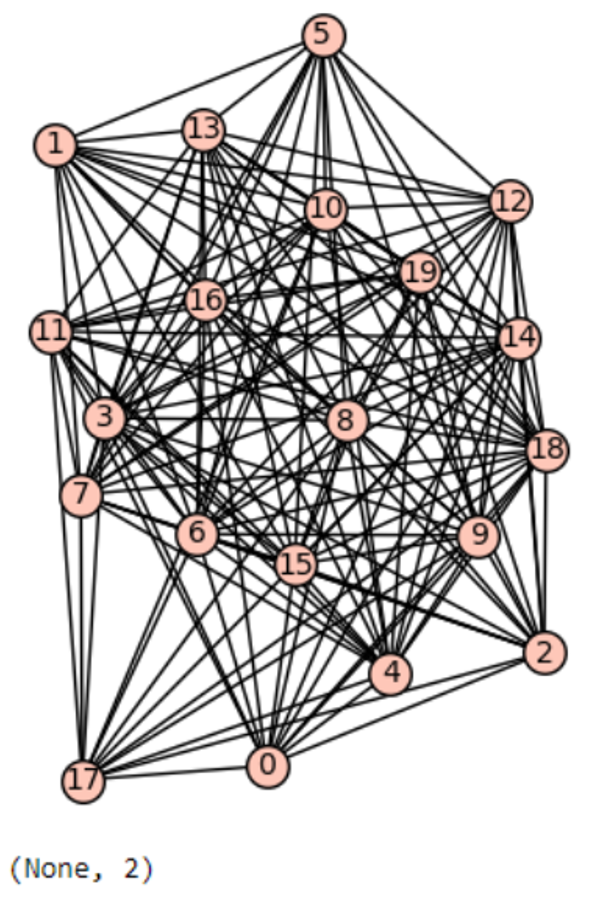
\includegraphics[width=5cm, height=6cm]{Slika5}
    \label{fig:mesh1}
\end{figure}\\
\begin{figure}[h!]
    \centering
    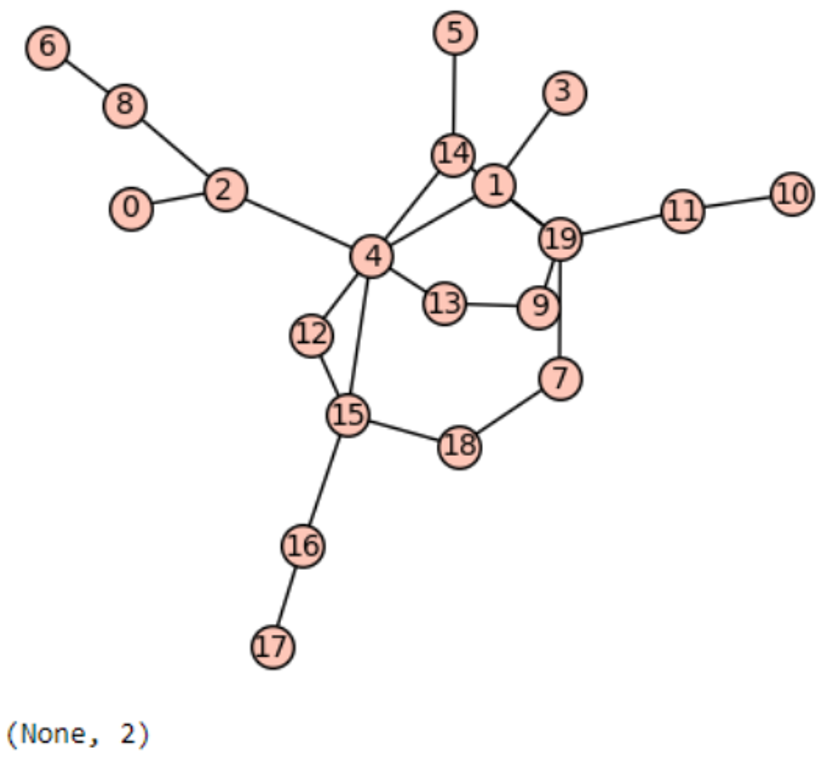
\includegraphics[width=5cm, height=5cm]{Slika6}
    \label{fig:mesh1}
\end{figure}\\

\subsection{Drevesa}

Poizkuse sva izvajala tudi na povezanih drevesih, katere sva lahko preverila v celoti na večjem številu vozlišč, saj jih je samih po sebi manj, kot pa npr. vseh možnih povezanih grafov na istem številu vozlišč. Testirala sva za $k$ med 4 in 12, ter število vozlišč do 20. Tu sva opazila, podobne stvari kot pri majhnih grafih, iz česar sklepava, da manj ko ima graf povezav(je podoben drevesu), večja je verjetnost, da se koeficient približa 2.\\

\subsection{Dvodelni grafi}
Posebej sva kodo izvajala še na dvodelnih drevesih z vozlišči $n \in \{1, \cdots, 20\}$, kjer sva ugotovila, da formula $\frac{n}{\lfloor{\frac{n}{2}}\rfloor}$ velja za vsa vozlišča od 1 do vključno s 3, nato pa je koeficient zmeraj enak 2.

\end{document}
